\section{Zielsetzung}
In diesem Versuch werden das Emissionsspektrum einer Kupfer-Röntgenröhre sowie diverse Absorptionsspektren aufgenommen und untersucht.

\section{Theorie}
\label{sec:Theorie}

Röntgenstrahlen werden erzeugt, in dem in einer evakuierten Röhre Elektronen aus einer Glühkathode beschleunigt werden.
Diese treffen auf eine Kupferanode. An dieser werden sie werden sie abgebremst und die verlorene kinetische Energie wird in Photonen umgewandelt. Entsteht ein kontinuierliches Bremsspektrum wie in \autoref{fig:theo-brems} zu sehen.

\begin{figure}
    \centering
    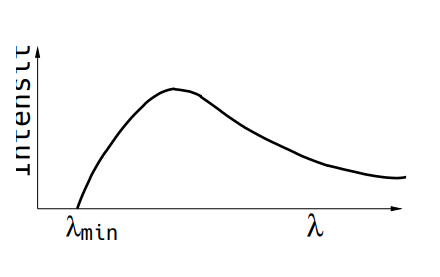
\includegraphics[width=0.8\textwidth]{content/bremsspektrum.PNG}
    \caption{Das Bremsspektrum einer Röntgenröhre, ohne Störeinflüsse und ohne das charakteristische Spektrum\cite{V602}.}
    \label{fig:theo-brems}
\end{figure}

Die Kontinuität urt daher, dass die Elektronen sowohl einen Teil ihrer kinetischen Energie wie auch die gesamte kinetische Energie abgeben können.
Geben sie ihre gesamte Energie ab, so hat der Lichtquant entsprechend die minimale Wellenlänge

\begin{equation}
    \label{eqn:lambda-min}
    \lambda_\text{min} = \frac{h c}{e_0 U}.
\end{equation}

Dabei ist $h$ das Planck'sche Wirkungsquantum und $c$ die Lichtgeschwindigkeit.
Das kontinuierliche Spektrum wird des Weiteren von einem charakteristischen Spektrum überlagert.
Dieses entsteht, wenn die Elektronen ein Atom ionisieren. Anschließend fällt ein Elektron aus einer höheren Schale herunter und emittiert ein Photon mit einer materialspezifischen Energie.
Die Frequenz dieses Photons wird mittels

\begin{equation}
    \label{eqn:schalen}
    E_\text{m} - E_\text{n} = h \nu
\end{equation}

berechnet, wobei $E_\text{m}$ und $E_\text{n}$ die jeweiligen Energieniveaus im Atom sind.
Das charakteristische Spektrum zeigt sich als stark ausgeprägte, scharfe Linien.
Dabei gilt für die Bindungsenergie

\begin{equation}
    \label{eqn:Bindungsenergie}
    E_\text{n} = -R_\infty z_\text{eff}^2 \cdot \frac{1}{n^2}.
\end{equation}

Dies liegt daran, dass die Wechselwirkung der Elektronen untereinander die Coulomb-Kraft zum Kern hin abschirmt.
Hierbei ist $R_\infty = 13.6$ eV die Rydbergenergie, $\sigma$ die Abschirmkonstante und $z_\text{eff} = z - \sigma$ die effektive Kernladung.
Es ist zu beachten, dass sich die Abschirmkonstante für jedes einzelne Elektron unterscheidet.
Auch da die äußeren Elektronen sich im Bahndrehimpuls und im Spin unterscheiden, sind die charakteristischen Linien in der Regel eher sehr eng beieinander liegende feinere Linien.

Bei Absorption von Röntgenstrahlen mit Energien <1 MeV sind der Compton- sowie der Photoeffekt die dominanten Prozesse.
Dabei nimmt der Absorptionskoeffizient mit zunehmender Energie ab und steigt sprunghaft, wenn die Photonenenergie gerade groß genug ist, um ein Atom zu ionisieren.
Daraufhin fällt er erneut ab, bis ein Elektron aus der nächsten Schale herausgestoßen werden kann.

Die hierbei auftretenden Bindungsenergien $E_\text{n,j}$ eines Elektrons lassen sich hier mittels der Sommerfeld'schen Feinstrukturformel 

\begin{equation}
    \label{eqn:fein-struktur}
    E_\text{n,j} = -R_\infty \bigg( z_\text{eff,1}^2 \cdot \frac{1}{n^2} + \alpha^2 z_\text{eff,2}^4 \cdot \frac{1}{n^3} \bigg( \frac{1}{j + \frac{1}{2}} - \frac{3}{4n} \bigg) \bigg)
\end{equation}

berechnen. Dabei ist $\alpha$ die Sommerfeld'sche Feinstrukturkonstante, $n$ die Hauptquantenzahl und $j$ der Gesamtdrehimpuls des jeweiligen Elektrons.

Die Abschirmkonstante lässt sich über die Energiedifferenz von zwei $L$-Kanten bestimmt werden. 
Da in diesem Versuch allerdings die ersten zwei Kanten nicht aufgelöst werden können, 
sodass die Energiedifferenz $\L$ $\Delta E_\text{L} = E_\text{L,II} - E_\text{L,III}$ verwendet wird.

Somit berechnet sich die Abschirmkonstante wie folgt:

\begin{equation}
    \label{eqn:abschirm}
    \sigma_\text{L} = Z - \bigg( \frac{4}{\alpha} \sqrt{\frac{\Delta E_\text{L}}{R_\infty }} - \frac{5 \Delta E_\text{L}}{R_\infty} \bigg)^\frac{1}{2} \cdot \bigg( 1 + \frac{19}{32} \alpha^2 \frac{\Delta E_\text{L}}{R_\infty} \bigg)^\frac{1}{2}.
\end{equation}

Die Energie eines Röntgenquants wird experimentell mittels Bragg'scher Reflexion bestimmt.
Dabei wird das Licht an einem Kristall reflektiert und es entsteht bei einem Glanzwinkel $\theta$ konstruktive Interferenz.
Ist die Gitterkonstate $d$ des Kristalls bekannt, kann die zum Winkel gehörige Wellenlänge über die Bragg'sche Bedingung

\begin{equation}
    \label{eqn:bragg}
    2 d \sin (\theta) = n \lambda
\end{equation}

berechnet werden. Dabei ist $n$ die Ordnung, bei der die Interferenz auftritt.
Über den Zusammenhang $E = h \nu$ lässt sich die Bragg'sche Bedingung auch als Energie abhängig von dem Winkel formulieren:

\begin{equation}
    \label{eqn:bragg-energie}
    E = \frac{h c}{2 d \sin (\theta )}.
\end{equation}
